\section*{4.1 Vector spaces and subspaces}
  \subsection*{Theory}

    \subsubsection*{Vector Space}
    \begin{mydef}\label{vector space}
      A vector space is a nonempty set $ V $ of objects, called vectors, on which are fefined two operations, called addition and multiplication by scalars (real numbers), subject to the ten axioms listed below. The axioms must hold for all vectors $ \mathbf u, \mathbf v $ and  $ \mathbf W $ in $ V $ and for all scalars $ c $ and $ d $.
      \begin{enumerate}
        \item The sum of $ u $ and $ v $, denoted by $ \mathbf u + \mathbf v $, is in $ V $
        \item $ \mathbf u + \mathbf v = \mathbf v + \mathbf u $
        \item $ (\mathbf u + \mathbf v) + \mathbf w = \mathbf u + (\mathbf v + \mathbf w)  $
        \item There is a zero vector $ \vec{0} $ in $ V $ such that $ \mathbf u + \mathbf 0 = u $
        \item For each $ \mathbf u $ in $ V $, there is a vector $ - \mathbf u $ in $ V $ such that $ \mathbf u + (-\mathbf u) = 0 $
        \item The scalar multiple of $ u $ by $ c $ denoted by $ c \mathbf u $ is in $ V $
        \item $ c (\mathbf{u + v}) = c \mathbf u + c \mathbf v $
        \item $ (c+d)\mathbf u = c \mathbf u + d \mathbf u $
        \item $ c(d \mathbf u) = (cd) \mathbf u $
        \item $ 1 \mathbf u  = \mathbf u $
      \end{enumerate}


    \end{mydef}

    \begin{mydef}\label{subspace}
      A subspace of a vector space V is a subset H of V that has three properties:
      \begin{itemize}
        \item The zero vector of V is in H
        \item $H$ is closed under vector addition. That is, for each $  \mathbf  u $ and $ \mathbf  v$ in $H$, the sum $ \mathbf  u$ $C$ $ \mathbf  v$
        is in $H$
        \item $H$ is closed under multiplication by scalars. That is, for each $ \mathbf  u$ in $H$ and each
        scalar $c$, the vector $c \mathbf  u$ is in $H$        
      \end{itemize}
    \end{mydef}

    \begin{theorem} \label{Theorem 1}
      If $ \vec{v_1}, \dots, \vec{v_n} ∈ V$ then $ span\{\vec{v_1}, \dots, \vec{v_n}\} $ is a subspace of $ V $ 
    \end{theorem}

  \subsection*{Exercises}
    \subsubsection*{12}

    Let $ W $ be the set of all vectors of the form $   \begin{pmatrix}
         s + 3t   \\ 
         s - t \\ 
         2s - t \\
         4t
      \end{pmatrix} $. 
    Show that $ W $ is a subspace of $ \mathbb R^{4} $. \newline \newline 

    We can split $ W $ up into a sum of other vectors. 
    $$
        \begin{pmatrix}
          s + 3t   \\ 
          s - t \\ 
          2s - t \\
          4t
        \end{pmatrix} = 
     s   \begin{pmatrix}
          1  \\ 
          1  \\ 
          2  \\
          0  
       \end{pmatrix} + 
    t   \begin{pmatrix}
         3  \\ 
         -1  \\ 
         -1  \\
         4  
      \end{pmatrix}
    $$
    \[
    W = span \left\{
      \begin{pmatrix}
        1  \\ 
        1  \\ 
        2  \\
        0  
     \end{pmatrix} , 
     \begin{pmatrix}
       3  \\ 
       -1  \\ 
       -1  \\
       4  
    \end{pmatrix}
    \right\}_{}^{} → 
    \text{\cref{Theorem 1} says $ W $ is a subspace of $ \mathbb R^{4} $}
    \]

    \subsubsection*{40}
    Let $ H $ and  $ K $ be subspaces of a vector space $ V $. The intersection of $ H $ and $ K $, written $ H \bigcap K $ is a subspace of $ V $. Give an example in $ \mathbb R^{2}  $ to show that the union of two subspaces is not, in general, a subspace 
    \begin{figure}[h!]
      \centering
      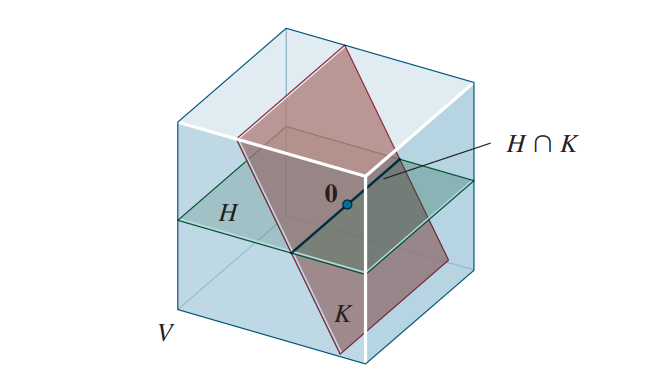
\includegraphics[scale = .7]{Bilder/HK_intersect.png}
      \caption{}
      \label{fig:figure1}
    \end{figure}
    \newline \newline 

    If you lift the $ H $ plane, higher and would by definition \ref{subspace}, not be a subspace as the intersection wouldn't go through origin. We can do the same for two lines in $ \mathbb R^{2} $. If they do not intersect in the origin, then their intersection can't be a subspace. 

    \subsubsection*{44}
    Determine if $ \mathbf y $ is in the subspace of $ \mathbb R^{4} $ spanned by the collumns of $ A $, where
    \[
    \mathbf y = 
    \begin{pmatrix}
       -4  \\ 
       -8  \\ 
       6  \\
       -5  
    \end{pmatrix}, \quad
    A = \begin{pmatrix}
      3 & -5 & -9 \\ 
      8 & 7 & -6 \\ 
      -5 & -8 & 3 \\ 
      2 & -2 & -9
    \end{pmatrix}
    \]
    \newline \newline 
    We can divide $ A $ into three vectors where each one is a column in $ A $. If these three vectors can form a linear combination which can create $ \mathbf y $ (in other words, $ \mathbf y $ is in the span of these vectors), then $ \mathbf y $ will be in the subspace of $ \mathbb R^{4}$ spanned by the columns of $ A $. To test this we append the vector $ \mathbf y $ to the end of $ A $ and then reduce it to row echelon form. 
    \begin{figure}[h!]
      \centering
      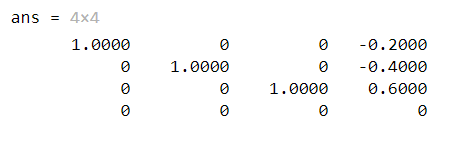
\includegraphics[scale = .7]{Bilder/Exercise_44_matlab.png}
      \caption{Results using matlab}
      \label{fig:figure1}
    \end{figure}
    As seen above the equation has a solution which means $ \mathbf  y $ is in the subspace of $ \mathbb R^{4}$ spanned by the columns of $ A $.

\section*{4.2 Null Spaces, Column Spaces, Row Spaces, and Linear Transformations}
  \subsection*{Theory}
    \subsubsection*{The Null Space of a Matrix}
    
    \begin{mydef}\label{def: null space}
      The \bf{null space} of an $ m × n $ matrix $ A $, written as Nul $ A $, is the set of all solutions of the homogenous equation $ A \mathbf x = \mathbf 0 $. In set notation, 
      \[
      \text{Nul} \ A = \left\{\mathbf x: \mathbf x \text{is in $ \mathbb R^{n} $ and $ A \mathbf X = \mathbf 0 $}\right\}_{}^{} 
      \]
    \end{mydef}    

    \begin{figure}[h!]
      \centering
      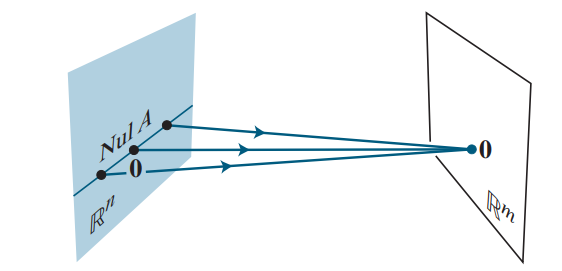
\includegraphics[scale = .7]{Bilder/nullspace_figure.png}
      \caption{Visualization of the subspace (in this case a line) formed by the null space of $ A $}
      \label{fig:figure1}
    \end{figure}

    \begin{theorem} \label{theorem: null space}
      The null space of an $ m × n  $ matrix $ A $ is a subspace of $ \mathbb R^{n} $. Equivalentrly, the set of all solutions to a system $ A \mathbf  x = \mathbf  0 $ of $ m  $ homogeneous linear equations in $ n $ unknowns is a subspace of $ \mathbb R^{n} $. 
    \end{theorem}

    \subsubsection*{The Column Space of a Matrix}
      \begin{mydef}\label{def: column space}
        The Column space of an $ m × n $ matrix $ A $, written as Col $ A $, is the set of all linear cominations of the collumns of $ A $. If $ A = \left[\mathbf a_1 \dots \mathbf a_n\right]_{}^{} $, then 
        \[
        Col \ A = Span = \left\{\mathbf a_1 \dots \mathbf a_n\right\}_{}^{} 
        \]
      \end{mydef}

      \begin{theorem}\label{theorem: column space}
        The column space of an $ m × n $ matrix $ A $ is a subspace of $ \mathbb R^{n} $. 
      \end{theorem}

    \subsection*{Exercises}
      \subsubsection*{4}
        Find the explicit definition of Nul $ A $ by listing vectors that span the null space. 
        \[
        A = \begin{bmatrix}
          1 & -6 & 4 & 0\\ 
          0 & 0 & 2 & 0
        \end{bmatrix}
        \]
        We start by reducing it to echelon form multiplying by $ \mathbf x $ and set as equal to the zero vector. 
        \[
        A \mathbf x = \mathbf 0
        \]
        \[
        rref(A) = \begin{bmatrix}
          1 & -6 & 0 & 0\\ 
          0 & 0 & 1 & 0
        \end{bmatrix}
        \]
        \[
          \begin{bmatrix}
            1 & -6 & 4 & 0\\ 
            0 & 0 & 2 & 0
          \end{bmatrix} 
          \mathbf x = 
          \begin{pmatrix}
             0  \\ 
             0 
          \end{pmatrix}
        \]
        \[
        \mathbf x = \begin{pmatrix}
           0  \\ 
           0  \\ 
           0  \\
           0  
        \end{pmatrix}
        \]
        \[
        Nul \ A = span \left\{\begin{pmatrix}
          0  \\ 
          0  \\ 
          0  \\
          0  
       \end{pmatrix}\right\}_{}^{} 
        \]
    
    \subsubsection*{52}
      Let $ H = Span\{\mathbf v_1, \mathbf v_2\} $ and $ K = Span\{\mathbf v_3, \mathbf v_4\}$, where 
      \[
      \mathbf v_1 = \begin{pmatrix}
         5  \\ 
         3  \\ 
         8 
      \end{pmatrix}, 
      \mathbf v_2 = \begin{pmatrix}
         1  \\ 
         3  \\ 
         4 
      \end{pmatrix}, 
      \mathbf v_3 = \begin{pmatrix}
         2  \\ 
         -1  \\ 
         5 
      \end{pmatrix}, 
      \mathbf v_4 = \begin{pmatrix}
         0  \\ 
         -12  \\ 
         -28 
      \end{pmatrix} 
      \]
      Then $ H $ and $ K $ are subspaces of $ \mathbb R^{3} $. In fact, $ H $ and $ K $ are planes in $ \mathbb R^{3} $ through origin, and they intersect in a line through $ \mathbf 0 $. Find a nonzero vector $ \mathbf w $ that generates that line. [Hint: $ \mathbf w $ can be written as $ c_1 \mathbf v_1 + c_2 \mathbf v_2 $ and also as $ c_3 \mathbf v_3 + c_4 \mathbf v_4 $. To build $ \mathbf w $, solve the equation $ c_1 \mathbf v_1 + c_2 \mathbf v_2  = c_3 \mathbf v_3 + c_4 \mathbf v_4  $ for the unknown $ c_j $'s] \newline \newline 




    